\subsubsection{Decoherence}\label{sec:decoherence}

In the previous section, we introduced decoherence as the gradual loss of the quantum properties of a qubit due to interactions with the surrounding environment (\autopageref{sec:why-quantum-computers-are-noisy}). Now, the natural question is: \textbf{\emph{how does decoherence actually modify a quantum state?}} To understand this, we need to introduce two types of errors, because decoherence can manifest itself in different ways.

\longline

\paragraph{Phase-Flip Errors}\label{sec:phase-flip-errors}

One common consequence of decoherence is \definition{Dephasing}, also called \definition{Loss of Phase}.

\highspace
Consider the qubit:
\begin{equation*}
    \ket{\psi} = \frac{\ket{0} + \ket{1}}{\sqrt{2}} = \ket{+}
\end{equation*}
The probabilities are:
\begin{equation*}
    P(0) = \left|\frac{1}{\sqrt{2}}\right|^2 = \frac{1}{2} \qquad P(1) = \left|\frac{1}{\sqrt{2}}\right|^2 = \frac{1}{2}
\end{equation*}
The important observation is that a quantum state contains more information than probabilities. It \hl{also contains the \textbf{relative phase} between the amplitudes}. For example, the states:
\begin{equation*}
    \ket{+} = \frac{\ket{0} + \ket{1}}{\sqrt{2}} \qquad \ket{-} = \frac{\ket{0} - \ket{1}}{\sqrt{2}}
\end{equation*}
Have exactly the same probabilities:
\begin{equation*}
    P(0) = P(1) = \frac{1}{2}
\end{equation*}
However, they \textbf{behave differently} in interference experiments because their \textbf{relative phase is different}.

\highspace
\textcolor{Green3}{\faIcon{question-circle} \textbf{What does Dephasing do?}} And, \textcolor{Red2}{\faIcon{exclamation-triangle} \textbf{why is it hard to notice?}} During dephasing, the \textbf{probabilities remain unchanged}, but the \textbf{relative phase becomes randomized}. This means that:
\begin{itemize}
    \item \hl{The \textbf{coherence} between the states \textbf{is lost}.}\phantomsection\label{def:coherence}

    \textcolor{Green3}{\faIcon{question-circle} \textbf{What is Coherence?}} A quantum state is \definitionWithSpecificIndex{coherent}{Coherent Quantum State}{} if the \textbf{different components} of the superposition \textbf{maintain a fixed phase relationship}.

    For example:
    \begin{equation*}
        \ket{\psi} = \frac{\ket{0} + \ket{1}}{\sqrt{2}} \quad \ket{\psi} = \frac{\ket{0} - \ket{1}}{\sqrt{2}}
    \end{equation*}
    Are coherent states because the relative phase between $\ket{0}$ and $\ket{1}$ is well-defined. Also, the state:
    \begin{equation*}
        \ket{\psi} = \sqrt{0.8}\ket{0} + e^{i\pi/3}\sqrt{0.2}\ket{1}
    \end{equation*}
    Is also coherent because the relative phase between $\ket{0}$ and $\ket{1}$ is well-defined. The \textbf{amplitudes don't matter} for coherence, the important thing is that the \textbf{phase relationship is known and stable}.

    \textcolor{Green3}{\faIcon[regular]{lightbulb} \textbf{Wave analogy for coherence.}} The following figures should not be interpreted as the actual amplitudes of a qubit. They are only a visual analogy. The two waves represent the two components of a quantum superposition and \hl{illustrate whether their relative phase relationship remains stable over time.}

    \textcolor{Green3}{\faIcon{check-circle} \textbf{Coherent state.}} In a coherent quantum state, the relative phase between the \textbf{amplitudes remains well-defined and stable}. In the figure, the two waves remain perfectly synchronized: peaks align with peaks and valleys align with valleys. Although the amplitudes may evolve, their phase relationship is preserved. This stable phase relationship is what allows quantum interference to occur.
    \begin{center}
        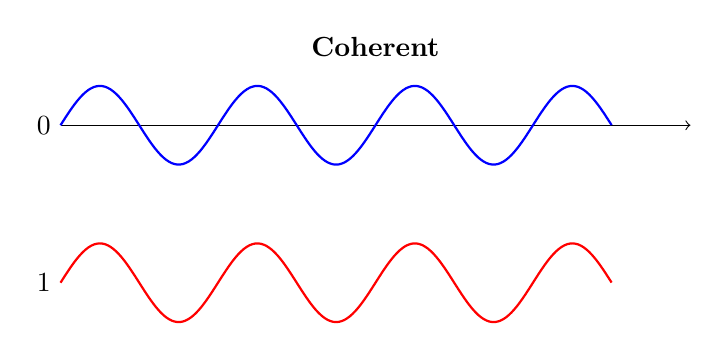
\begin{tikzpicture}
            \draw[->] (0,0) -- (8,0);

            \draw[blue,thick,samples=100,smooth,domain=0:7]
            plot(\x,{0.5*sin(180*\x)});

            \draw[red,thick,samples=100,smooth,domain=0:7]
            plot(\x,{0.5*sin(180*\x)-2});

            \node[left] at (0,0) {$\ket{0}$};
            \node[left] at (0,-2) {$\ket{1}$};

            \node at (4,1) {\textbf{Coherent}};
        \end{tikzpicture}
    \end{center}

    \textcolor{Red2}{\faIcon{exclamation-triangle} \textbf{Loss of Coherence.}} When a qubit interacts with its environment, the relative phase between the amplitudes gradually becomes uncertain. In the figure, the \textbf{two waves lose their synchronization over time}. The peaks and valleys no longer align, representing the loss of a well-defined phase relationship. This \textbf{gradual loss of phase synchronization is called \important{dephasing}} and is one of the main mechanisms responsible for decoherence. Once coherence is lost, interference effects disappear and the quantum state behaves more like a classical probabilistic system.

    \begin{center}
        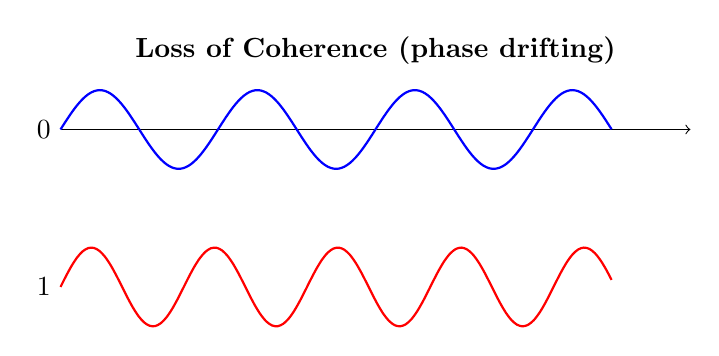
\begin{tikzpicture}
            \draw[->] (0,0) -- (8,0);

            \draw[blue,thick,samples=100,smooth,domain=0:7]
            plot(\x,{0.5*sin(180*\x)});

            \draw[red,thick,samples=100,smooth,domain=0:7]
            plot(\x,{0.5*sin(180*\x+50*\x)-2});

            \node[left] at (0,0) {$\ket{0}$};
            \node[left] at (0,-2) {$\ket{1}$};

            \node at (4,1) {\textbf{Loss of Coherence (phase drifting)}};
        \end{tikzpicture}
    \end{center}

    \textcolor{Red2}{\faIcon{exclamation-triangle} \textbf{Complete loss of coherence.}} If the \textbf{dephasing process continues}, the \textbf{relative phase becomes completely randomized}. In the figure, the two waves are no longer synchronized at all, and there is no stable phase relationship between them. This represents a fully decohered state, where the phase information has been completely lost. The system can no longer exploit quantum interference and therefore behaves similarly to a classical probabilistic mixture.
    \begin{center}
        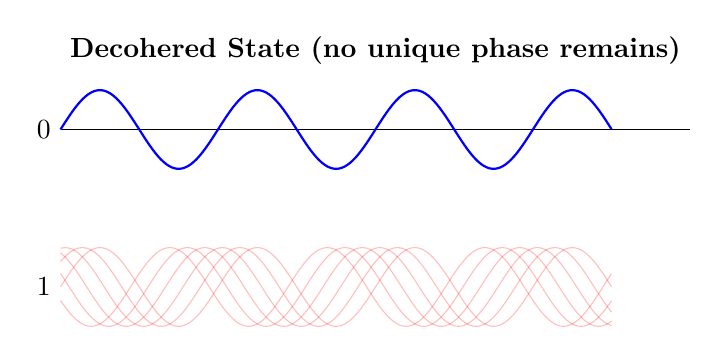
\begin{tikzpicture}
            \draw (0,0) -- (8,0);

            \draw[blue,thick,samples=100,smooth,domain=0:7]
            plot(\x,{0.5*sin(180*\x)});

            \foreach \p in {0,40,80,120,160,200}{
                \draw[red,opacity=0.25,samples=100,smooth,domain=0:7]
                plot(\x,{0.5*sin(180*\x+\p)-2});
            }

            \node[left] at (0,0) {$\ket{0}$};
            \node[left] at (0,-2) {$\ket{1}$};

            \node at (4,1) {\textbf{Decohered State (no unique phase remains)}};
        \end{tikzpicture}
    \end{center}

    \textcolor{Red2}{\faIcon{exclamation-triangle} \textbf{Classical Mixture.}} After \textbf{complete decoherence}, \textbf{all phase information is lost}, and the \textbf{quantum state can be described as a classical mixture of states}. In this case, the system behaves as if it were in state $\ket{0}$ with probability $50\%$ and in state $\ket{1}$ with probability $50\%$. The state no longer exhibits any quantum interference effects and can be treated as a classical probabilistic system. A great analogy is a coin that before the decoherence process was in a superposition of heads and tails, but after decoherence, it behaves like a classical coin that is either heads or tails with certain probabilities.
    \begin{center}
        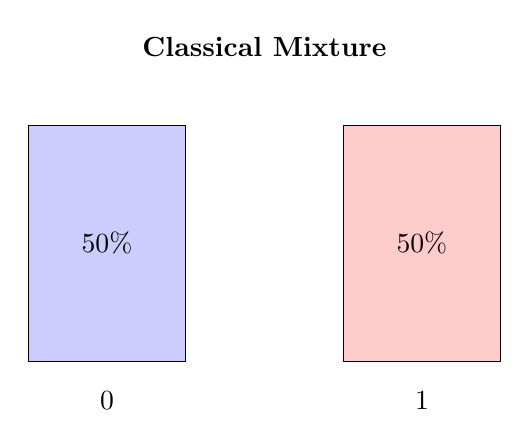
\begin{tikzpicture}
            \draw[fill=blue!20] (0,0) rectangle (2,3);
            \draw[fill=red!20] (4,0) rectangle (6,3);

            \node at (1,1.5) {$50\%$};
            \node at (5,1.5) {$50\%$};

            \node at (1,-0.5) {$\ket{0}$};
            \node at (5,-0.5) {$\ket{1}$};

            \node at (3,4) {\textbf{Classical Mixture}};
        \end{tikzpicture}
    \end{center}

    Notice that this is \hl{fundamentally different from the coherent state}:
    \begin{equation*}
        \ket{+}
        =
        \frac{\ket{0}+\ket{1}}{\sqrt{2}}
    \end{equation*}
    Which also produces $50\%$ probabilities when measured. The difference is that the \textbf{coherent state contains phase information and can exhibit interference}, whereas the classical mixture contains only probabilities. 
    
    In summary, a coherent quantum state and a classical probabilistic mixture \textbf{may produce the same measurement probabilities}, but \hl{only the coherent state contains phase information and can therefore exhibit interference effects.}
    

    %%%%%%%%%%%%%%%%%%%%%%%%%%%%%%%%%

    
    \item \hl{Interference effects disappear.}\phantomsection\label{def:interference}

    \textcolor{Green3}{\faIcon{question-circle} \textbf{What is Interference?}} In the previous point, we mentioned that the loss of coherence leads to the disappearance of interference effects. \emph{But what exactly are interference effects?} \definition{Interference} is the \textbf{phenomenon by which quantum amplitudes combine}.

    Unlike classical probabilities, which simply add together, quantum amplitudes can be positive, negative or complex. Therefore, when \textbf{amplitudes are added} together, they can either \textbf{reinforce each other} (called \definition{Constructive Interference}) or \textbf{cancel each other out} (called \definition{Destructive Interference}).

    An example of constructive interference is shown in the figure below. The two waves represent the two components of a quantum superposition. When they are in phase (peaks align with peaks and valleys align with valleys), their amplitudes reinforce each other, leading to a stronger overall amplitude, and therefore a higher probability of certain measurement outcomes (because probabilities are obtained by taking the square of the amplitude).

    \begin{center}
        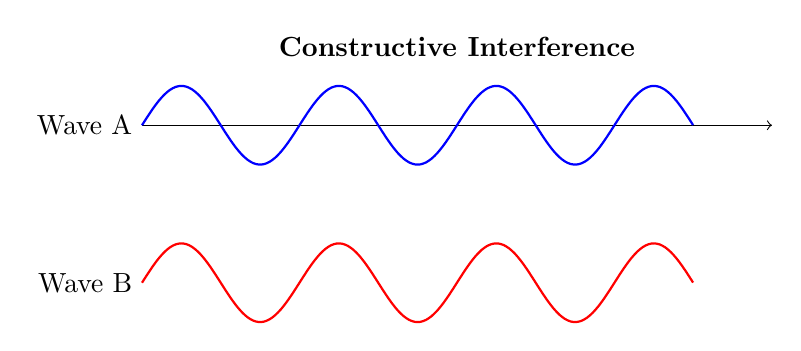
\begin{tikzpicture}
            \draw[->] (0,0) -- (8,0);

            \draw[blue,thick,samples=100,smooth,domain=0:7]
            plot(\x,{0.5*sin(180*\x)});

            \draw[red,thick,samples=100,smooth,domain=0:7]
            plot(\x,{0.5*sin(180*\x)-2});

            \node[left] at (0,0) {Wave A};
            \node[left] at (0,-2) {Wave B};

            \node at (4,1) {\textbf{Constructive Interference}};
        \end{tikzpicture}
    \end{center}

    On the other hand, when the two waves are out of phase (peaks align with valleys), their amplitudes cancel each other out, leading to a weaker overall amplitude, and therefore a lower probability of certain measurement outcomes.

    \begin{center}
        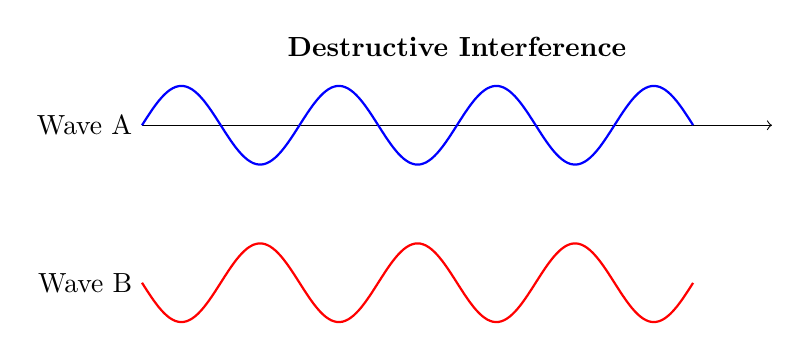
\begin{tikzpicture}
            \draw[->] (0,0) -- (8,0);

            \draw[blue,thick,samples=100,smooth,domain=0:7]
            plot(\x,{0.5*sin(180*\x)});

            \draw[red,thick,samples=100,smooth,domain=0:7]
            plot(\x,{-0.5*sin(180*\x)-2});

            \node[left] at (0,0) {Wave A};
            \node[left] at (0,-2) {Wave B};

            \node at (4,1) {\textbf{Destructive Interference}};
        \end{tikzpicture}
    \end{center}
    
    \textcolor{Red2}{\faIcon{exclamation-triangle} \textbf{Decoherence and interference.}} Decoherence does not necessarily destroy the probabilities immediately. Instead, it destroys the \textbf{phase information}. Without phase information, interference effects disappear, and the quantum state behaves more like a classical probabilistic system. 
    
    \item \hl{The state becomes more classical.} As coherence is lost and interference effects disappear, the quantum state gradually behaves more like a classical probabilistic mixture. In the limit of complete decoherence, the state can be described as a classical mixture of states, where the system is in one state with a certain probability and in another state with another probability.
\end{itemize}
Dephasing is \textbf{invisble in the computational basis} because the probabilities of measuring $\ket{0}$ or $\ket{1}$ remain unchanged. However, the damage only becomes visible when the algorihtm relies on interference effects, which require coherence. This is one reason why decoherence is so dangerous. It can silently destroy the relative phases of a state without affecting the measurement probabilities in the computational basis, making it \textbf{difficult to detect until it's too late}.

\highspace
\textcolor{Green3}{\faIcon{question-circle} \textbf{Which mathematical error changes the phase of a quantum state?}} In other words, \textbf{\emph{which mathematical error corresponds to dephasing?}} The answer is the Pauli-Z gate:
\begin{equation*}
    Z = \begin{bmatrix}
        1 & 0 \\
        0 & -1
    \end{bmatrix}
\end{equation*}
Which acts as follows:
\begin{equation*}
    Z\ket{0} = \ket{0} \qquad Z\ket{1} = -\ket{1}
\end{equation*}
Where the minus sign in front of $\ket{1}$ represents a phase shift of $\pi$ (or 180 degrees). It is more intuitive to see the effect of the Z gate on the Bloch sphere, \autopageref{fig:pauli-z-eigenstates}. However, with Pauli-Z, the probabilities of measuring $\ket{0}$ or $\ket{1}$ remain unchanged, but the relative phase between the two states is flipped. This is why it's called a \definition{Phase-Flip Error}.

\highspace
\textcolor{Red2}{\faIcon{exclamation-triangle} \textbf{Why is it dangerous?}} Per se, the Pauli-$Z$ gate is not dangerous, and a \textbf{single application does not destroy coherence}. For example, applying a Pauli-$Z$ gate transforms (\ket{+}) into (\ket{-}), but the resulting state is still perfectly coherent.

\highspace
However, in a real quantum computer the environment does not apply one neat Pauli-$Z$ gate. Instead, interactions with the environment introduce many random phase perturbations over time. These random phase changes can be modeled as phase-flip ($Z$) errors. As they accumulate, the relative phase between the components of a superposition becomes increasingly uncertain, producing \textbf{dephasing}. The consequence is the loss of coherence and, therefore, the disappearance of the interference effects on which quantum algorithms rely.

\highspace
\textcolor{Green3}{\faIcon{question-circle} \textbf{If the Pauli-Z gate is a valid quantum operation, why is it associated with errors?}} Let's clarify this point with an analogy. For example, when we write $\text{NOT}(0) = 1$, there is nothing wrong with the NOT operation. The gate is doing exactly what it's supposed to do. However, suppose our program says to store the value $0$ in a variable, but electrical noise flips the bit to $1$. Now the bit has undergone a NOT operation, but this is not what we intended. The NOT operation is a valid operation, but in this context, it represents an error because it changes the value in an unintended way. \hl{Exactly the same thing happens in quantum computing.}

\highspace
Suppose our algorithm contains $Z\ket{+} = \ket{-}$. We intentionally changed the phase, and everything is correct. However, suppose our algorithm says ``\emph{do nothing}'', but the \hl{environment interacts with the qubit and changes its phase.} The effect on the state is $\ket{+} \to \ket{-}$, which is exactly what a $Z$ gate would have done. Now, we call this a \textbf{phase-flip error} because the phase changed even though we never requested that operation. \hl{The $Z$ gate is a valid quantum operation, but in this context, it represents an error because it changes the phase in an unintended way.}